\subsection{Subsystem Integration}
\label{sec:subsystem_integration}
The integration of all the subsystems is centered around the control subsystem. In the following sections, the team will discuss how these integrations will occur as the design process was centered around creating individual black boxes for each system to work against.

\subsubsection{Sensing}

The sensing subsystem has three key components for the control subsystem to interact with: the linear actuator rail that the sensors are mounted to, the light bulb generating photons for the spectrometer to receive, and the photodiode circuitry.

\paragraph{Linear Actuator Rail} The sensors will be mounted to a carriage that may slide back and forth on the linear rail. The position of the carriage on the linear rail determines the wavelength of light sampled, and therefore the wavelength can be interpolated by the position of the stepper motor controlling the spectrometer carriage. It is a natural conclusion that the microcontroller will be able to direct the spectrometer to measure a specific wavelength by moving the stepper motor a certain number of predetermined steps. The microcontroller will sample the entire spectral range and compile this data to prepare to send to the web subsystem for processing. Since the other optics are solid-state, the position of the endmost beam will be fixed at or just outside of the fully retracted state of the rail. Since the rail makes 5um steps, and the arrangement and size of the beams are flexible, the spectrometer will be aligned such that the stepper motor will make the same number of steps every time, until the maximum range is reached.

\paragraph{Photodiode} The photodiode is a passive instrument that generates current depending on the flux density on the sensor. This flux density is based on the strength of the specific wavelength emission, separated by the diffraction grating. The current is connected to the sensing subsystem circuitry described in \ref{sec:sensing_subsystem}. This circuitry will proportionally convert the current to a voltage, and the output of the circuit will be connected to an analog-configured pin of the microcontroller, which will be taken as an input to the microcontroller's analog-to-digital converter. The ADC will convert the voltage to a value able to be measured in programming. The current (and by extension, voltage) level measured will be paired with the wavelength and transmitted by the MCU to the Amazon EC2 instance.

\paragraph{Tungsten Light Bulb} The Spectrometer works by raising the frequency emissions of the soil above the noise created by heat and other sources of light. It does this by drawing on power from the battery to illuminate the bulb, however the light bulb expends a lot of power. It will only need to be on during the scanning motion of the rail, to save energy and protect from unwanted glare.

% TODO: Justin look this WHOLE SUBSECTION over and check if it's accurate.
\subsubsection{Power} The charge controller will deliver voltage of the battery to the microcontroller via

\subsubsection{Web}
The web and control subsystems interact via two way WebSocket protocol (\ref{websocket_protocol}), which will utilize TCP (\ref{tcp_standard}) as the transport layer protocol. Section \ref{sec:controller_subsystem} talks about the format of the raw texts in the packets. The web subsystem will be deployed to a fixed domain so the memory of the control system can use a fixed host for the Socket server. The socket server will always start by processing the address information of the incoming socket, and grabbing previous data from the database accordingly. The socket server will process the data, storing it in the database for reporting on later. If necessary, the socket server will send a request to the plant bed to do some function. This is laid out in \autoref{fig:web-control-sequence}.

\begin{figure}[H]
    \caption{Web--Plant Bed Socket Integration Sequence Diagram}
    \centering
    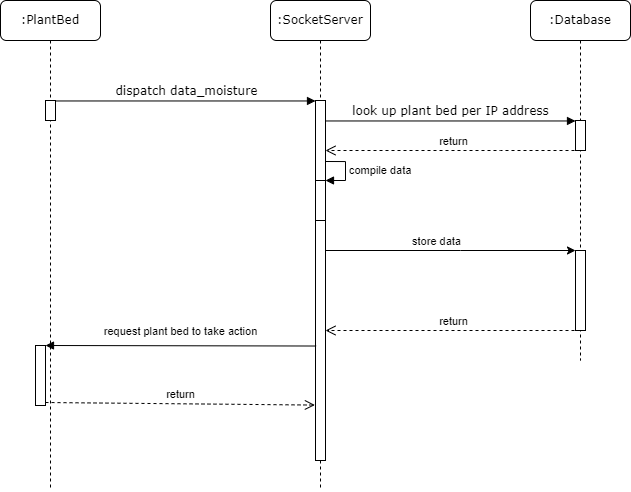
\includegraphics[width=.75\textwidth]{images/web-control-integration-sequence.png}
    \label{fig:web-control-sequence}
\end{figure}

